\section{Cyclic connectivity}\label{sec:snarks}


Let $G$ be a cubic graph and $S$ an edge-cut of size $n$. By severing the edges of $S$, we obtain two $n$-poles such that $G$ is a junction of them. If both contain a cycle, $S$ is said to be an \textit{n-edge-c-cut}. Generally, these edge cuts are called \textit{c-cuts}. 

A cubic graph $G$ is called \textit{cyclically n-edge-connected} if there is no c-cut with less than $n$ edges.
If $G$ has at least one c-cut, the \textit{cyclic edge connectivity} of $G$ is the smallest number of edges of a c-cut of $G$ and is denoted by $z(G)$.
The \textit{girth} of a graph $G$ is the minimum length of a cycle in $G$. If $G$ does not contain a cycle, we set the girth to $\infty$.

Many authors include in their definition of snarks additional criteria of \quotes{non-triviality}, for example, girth at least five or being cyclically-edge-4-connected \cite{Preissmann1983, Nedela1996}. On the other hand, some authors allow snarks to contain bridges \cite{IrreducibleSnarksSkoviera}, making the dumbbell graph on two vertices the smallest snark (\cref{fig:dumbbell}).

\begin{figure}
	\centering
	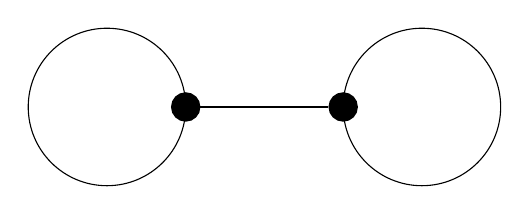
\begin{tikzpicture}[every node/.style={draw,circle,very thick, fill=black}]
	\node[shape=circle,draw=black] (1) at (0,0) {};
	\node[shape=circle,draw=black] (2) at (2,0) {};
	
	\path 
	(1) edge (2)
	;
	
	\draw (-1,0) circle [radius=1];
	\draw (3,0) circle [radius=1];
\end{tikzpicture}
	\caption{Dumbbell graph}
	\label{fig:dumbbell}
\end{figure}

The Petersen graph is the smallest snark satisfying every definition (\cref{fig:petersen}). Other notable snarks are the Blanuša snarks, or the infinite family of flower snarks discovered by R. Isaacs \cite{Isaacs1975}. The Isaacs snarks are denoted by $J_k$, where $k$ is an odd integer $k\geq 3$.

\begin{figure}
	\centering
	\begin{tikzpicture}[every node/.style={draw,circle,very thick, fill=black}]
	\graph[clockwise, radius=2cm, empty nodes] {subgraph C_n [n=5,name=A] };
	\graph[clockwise, radius=1cm, empty nodes] {subgraph I_n [n=5,name=B] };
	
	\foreach \i [evaluate={\j=int(mod(\i+2+4,5)+1)}]% using Paul Gaborit's optimisation
	in {1,2,3,4,5}{
		\draw (A \i) -- (B \i);
		\draw (B \j) -- (B \i);
	}
\end{tikzpicture}
	\caption{Petersen graph}
	\label{fig:petersen}
\end{figure}